\documentclass[10pt]{beamer}
\usetheme[outer/progressbar=foot]{metropolis}
\usepackage{booktabs}
%\usepackage[scale=2]{ccicons}
\usepackage{pgfplots}
\usepackage{cancel}
\usepackage[ngerman]{babel}
\usepackage[utf8]{inputenc}
\usepackage{blindtext}
\usepackage{amsmath}
\usepackage[italicdiff]{physics}
\usepackage[italic]{hepnames}
\usepackage{graphicx}
\usepackage{float}
\usepackage{color}
\usepackage{physics}
\usepackage{tikz}
\usepackage[absolute,overlay]{textpos}
%\usepackage[texcoord,grid,gridcolor=red!10,subgridcolor=green!10,gridunit=pt]{eso-pic}

\usepgfplotslibrary{dateplot}


%Frontpage
\title{Calorimetry and Deep Learning}
\date{\today}
\author{Simon Schnake}
\institute{Universität Hamburg}

%Document
\begin{document}
\maketitle
\tikzstyle{every picture}+=[remember picture]

\begin{frame}{Calorimetry in Particle Physics}
  \begin{columns}
    \column{0.5\textwidth}
    \begin{itemize}
    \item apparatus to measure the energy of a particle
    \item destructive process
    \item particle shower
    \item sampling or homogenous
    \item electromagnetic calorimeter \\
      $\rightarrow$ via EM interaction
    \item hadronic calorimeter \\
      $\rightarrow$ via strong nuclear force
    \item $\frac{\sigma_E}{E} \propto \frac{1}{\sqrt{E}}$
    \end{itemize}
    \column{0.5\textwidth}
    \begin{figure}[htp]
      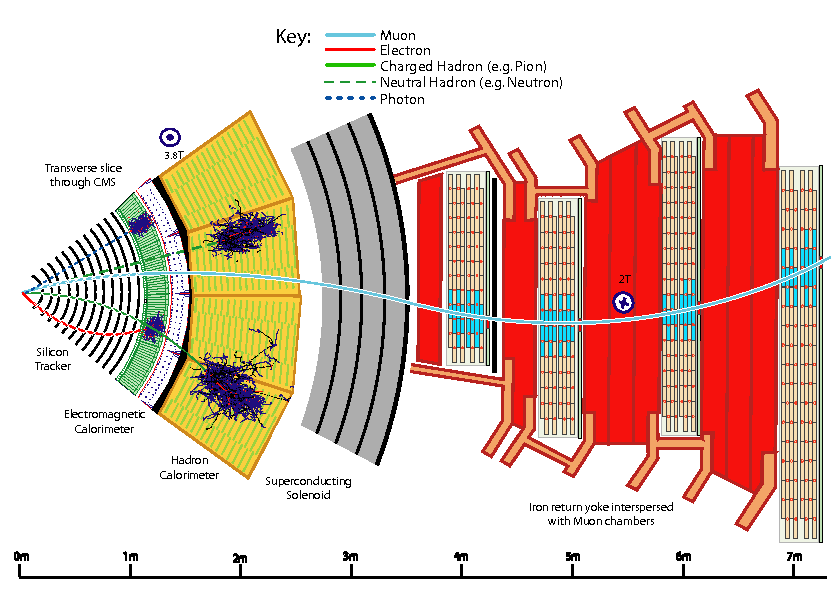
\includegraphics[width=2\textwidth]{Figure_001.png}
    \end{figure}

  \end{columns}
\end{frame}

\begin{frame}{Deep Learning}
  \begin{textblock*}{150pt}(200pt,35pt)
    \begin{figure}[htp]
      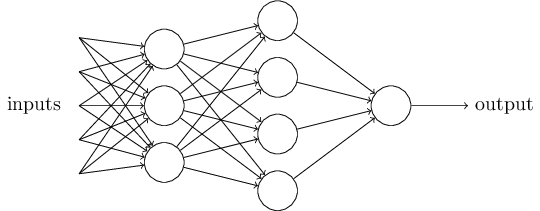
\includegraphics[width=\textwidth]{tikz1.png}
    \end{figure}
  \end{textblock*}
  \begin{itemize}
  \item Neuron: $\sigma_i(W_i X_{i-1}+b_{i})$
  \item Goal: Fitting NeuralNet($X_0$) to\  $y_{\text{true}}$
  \item Procedure:
    \begin{itemize}
    \item Define $Loss(y_{\text{true}}, y_{\text{pred}})$ to minimize
    \item Use Backpropagation to update $W_i, b_i$ via an optimizer
    \end{itemize}
  \end{itemize}
\end{frame}

\begin{frame}{Simulation Setup}
  \begin{columns}
    \column{0.5\textwidth}
    \begin{textblock*}{150pt}(2pt,55pt)
      \begin{itemize}
      \item Simulation with Geant4\small{}
      \item $e^-$ from 0. to 10 GeV
      \item 300,000 events
      \end{itemize}
    \end{textblock*}
    \begin{textblock*}{10pt}(2pt,125pt)
      \begin{tabular}{l|l|l}
        layer  & scint    & absorber \\ \hline
        layer 0      & 9mm     & 40 mm SS\\
        layer 1 - 8  & 3.7mm   & 50.5 mm brass \\
        layer 9 - 14 & 3.7mm   & 56.5 mm brass \\
        layer 15     & 3.7 mm  & 75 mm SS \\
        layer 16     & 9mm     &                      
      \end{tabular}
    \end{textblock*}
    \column{0.5\textwidth}
    \begin{figure}[htp]
      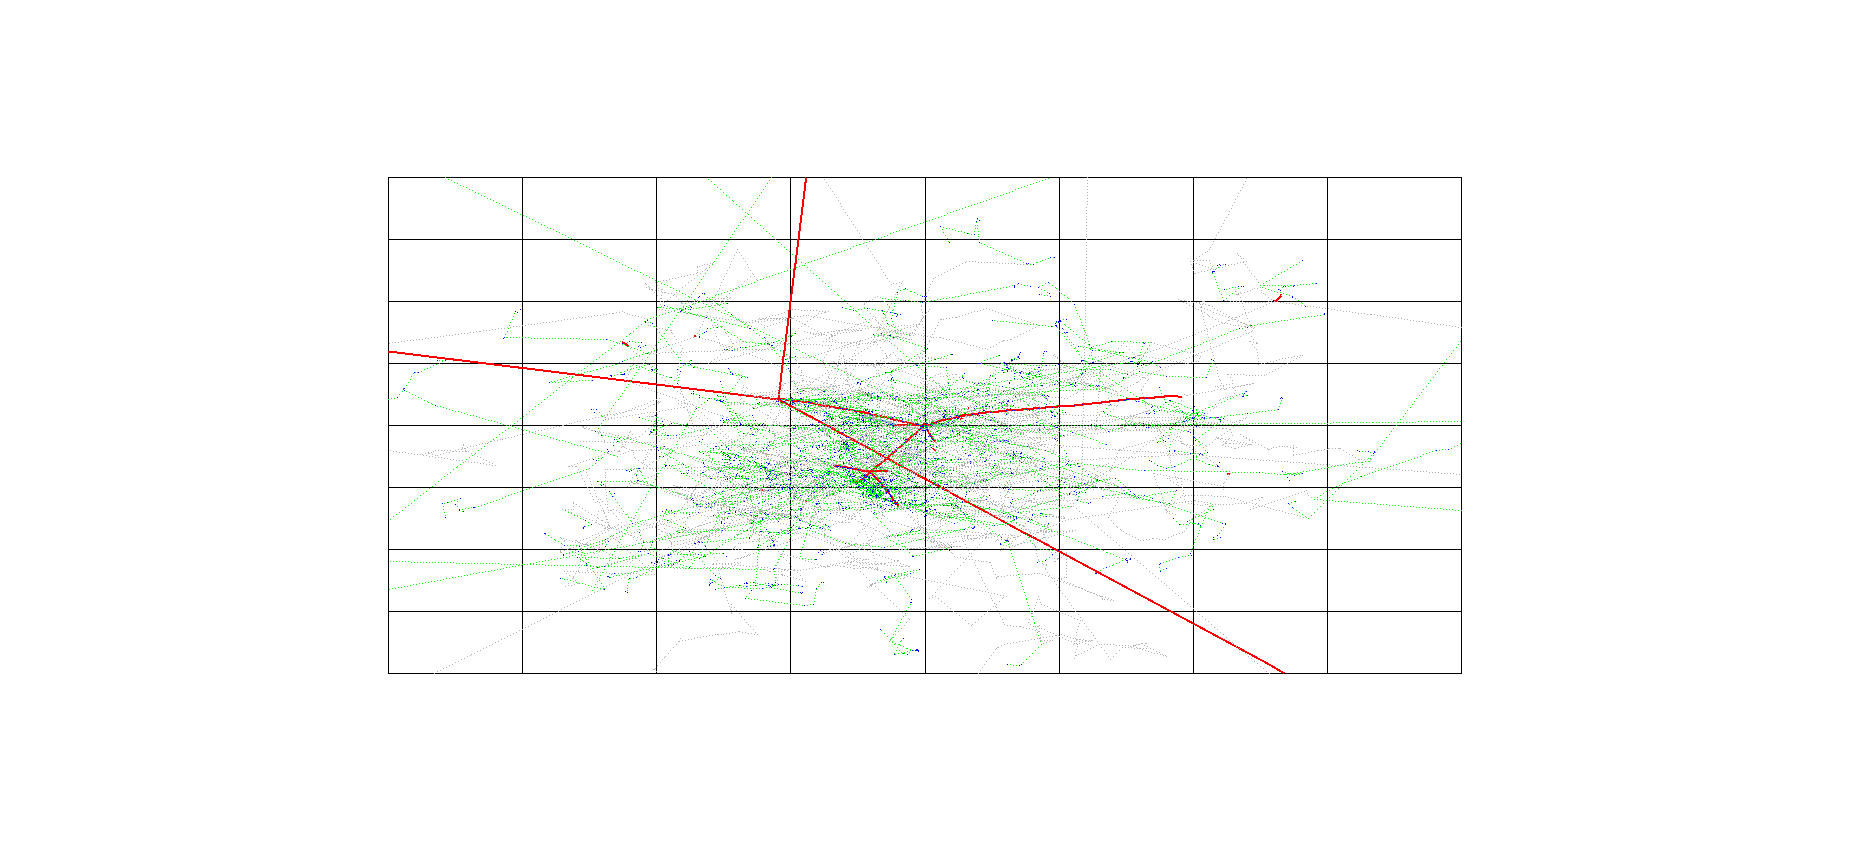
\includegraphics[width=1.1\textwidth]{front.png}\\
      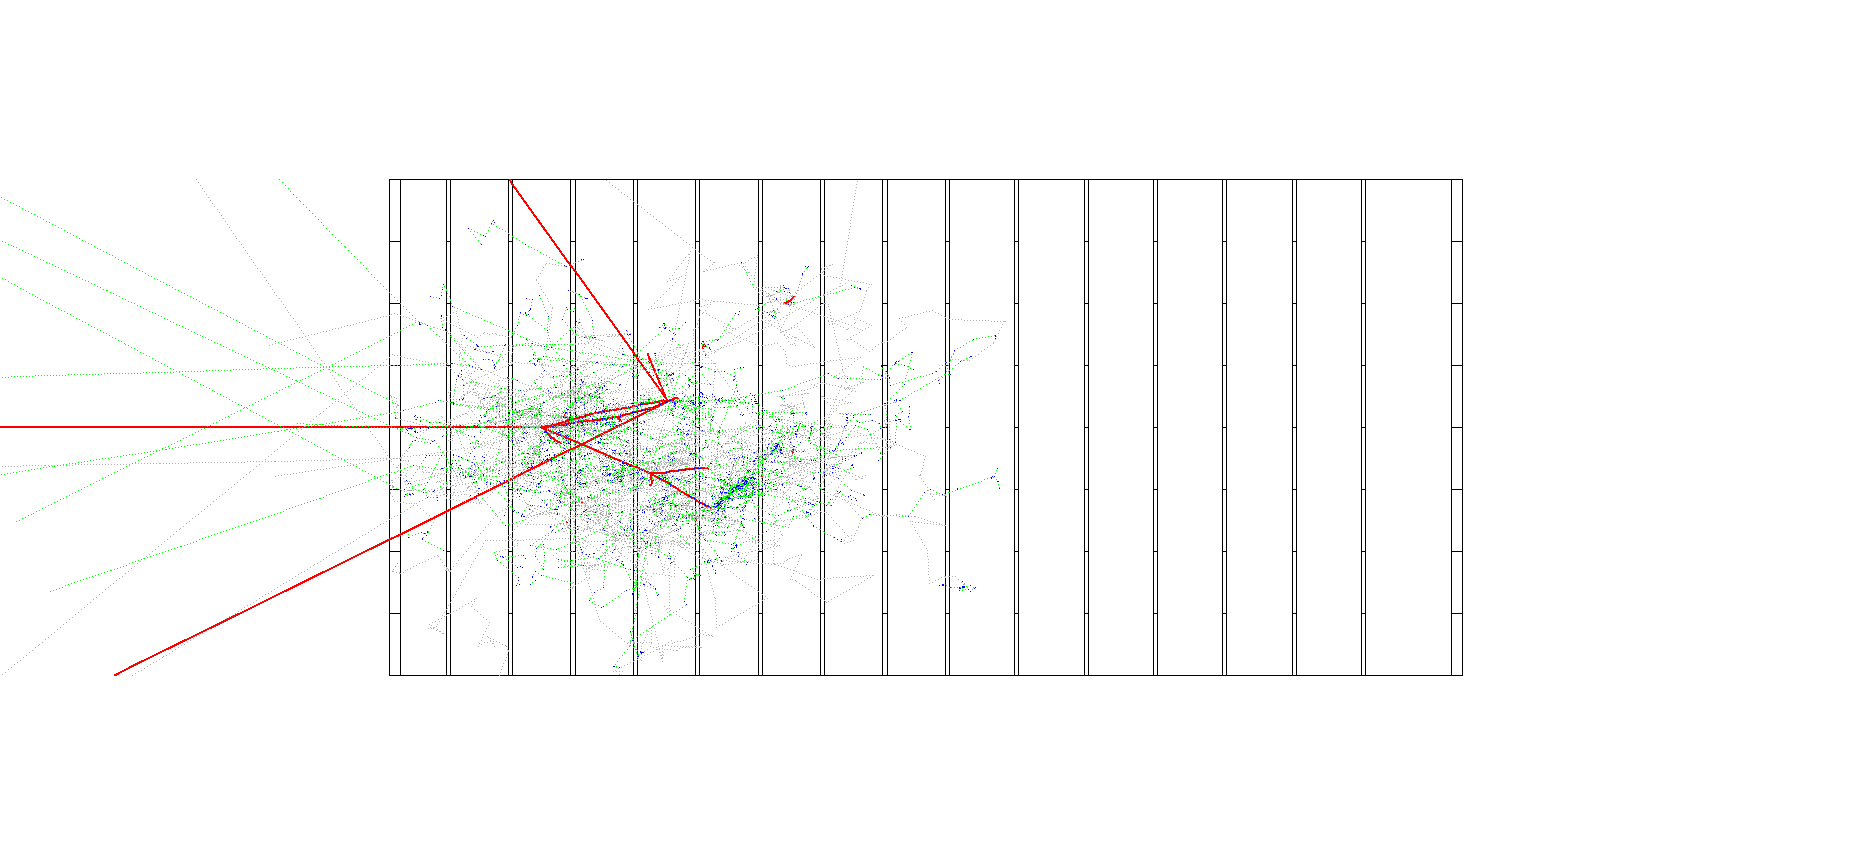
\includegraphics[width=1.1\textwidth]{side.png}
    \end{figure}
  \end{columns}
  \begin{textblock*}{100pt}(250pt,70pt)
    Front view
  \end{textblock*}
  \begin{textblock*}{100pt}(250pt,150pt)
    Side view
  \end{textblock*}
\end{frame}

\begin{frame}{Resulting Data}
  \begin{columns}
    \column{0.5\textwidth}
    \begin{figure}[htp]
      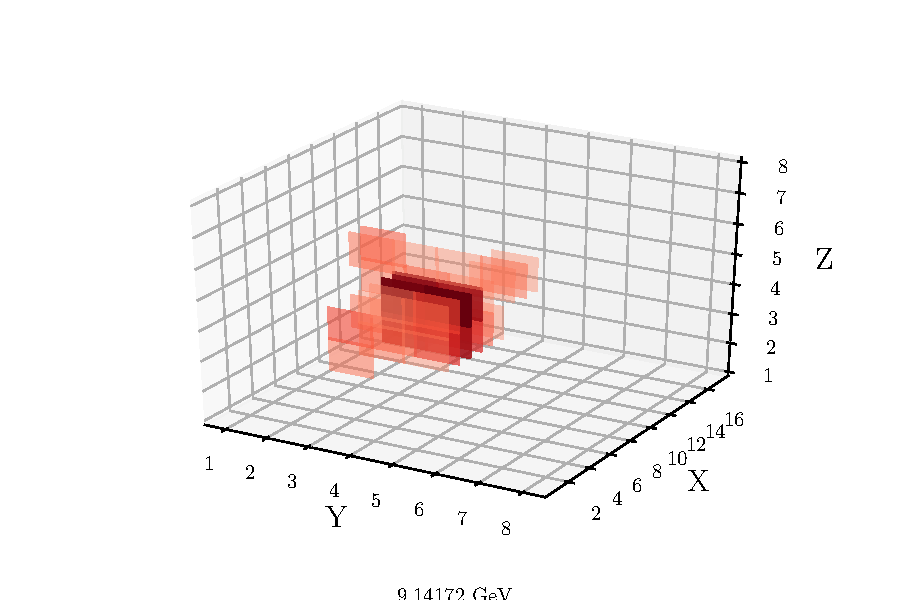
\includegraphics[width=1.1\textwidth]{../data_display.pdf}
    \end{figure}
    \column{0.5\textwidth}
    \begin{figure}[htp]
      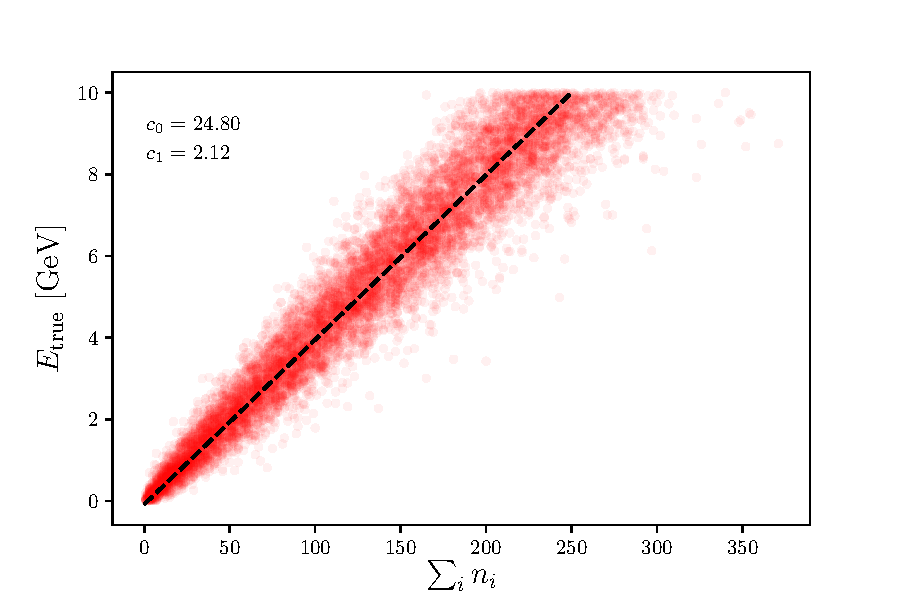
\includegraphics[width=\textwidth]{../e-vs-sum_n_fit.pdf}
    \end{figure}
  \end{columns}
\end{frame}

\begin{frame}{Neuralnet}
  \begin{tabular}{l|l|l}
    Layer & Type                                & Activation \\ \hline
    1     & Conv2D(32, (2,2), strides = (1, 1)) & ReLu       \\
    2     & Flatten()                           &            \\
    3-5   & Dense(128)                          & ReLu       \\
    6     & Dense(10)                           & ReLu       \\
    7     & Dense(1)                            & Linear    
  \end{tabular}
  \begin{itemize}
  \item Loss = Mean Squared Error
  \item Optimizer = RMSprop
  \end{itemize}
\end{frame}

\begin{frame}{First Results of the Neuralnet}
  \begin{columns}
    \column{0.5\textwidth}
    \begin{figure}[htp]
      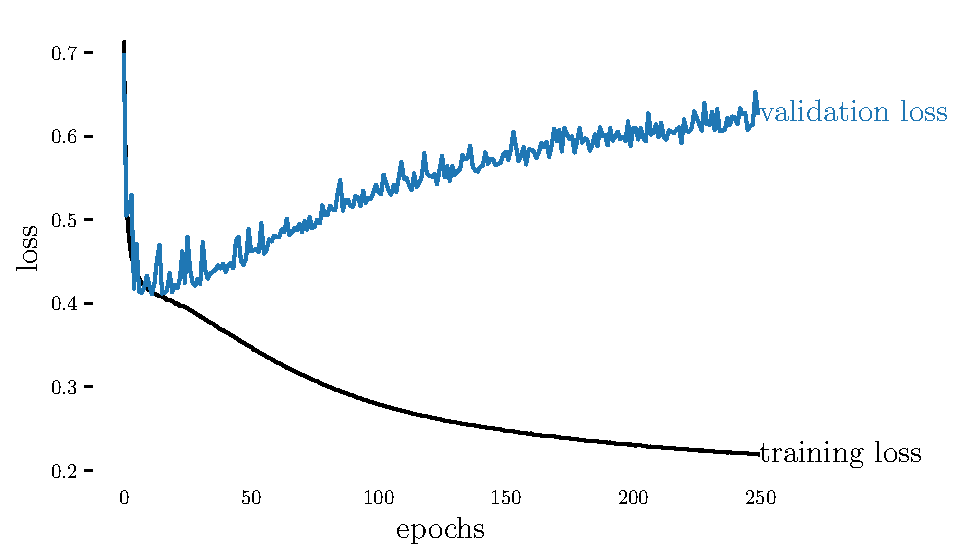
\includegraphics[width=1.1\textwidth]{../first_loss.pdf}
    \end{figure}
    \column{0.5\textwidth}
    \begin{figure}[htp]
      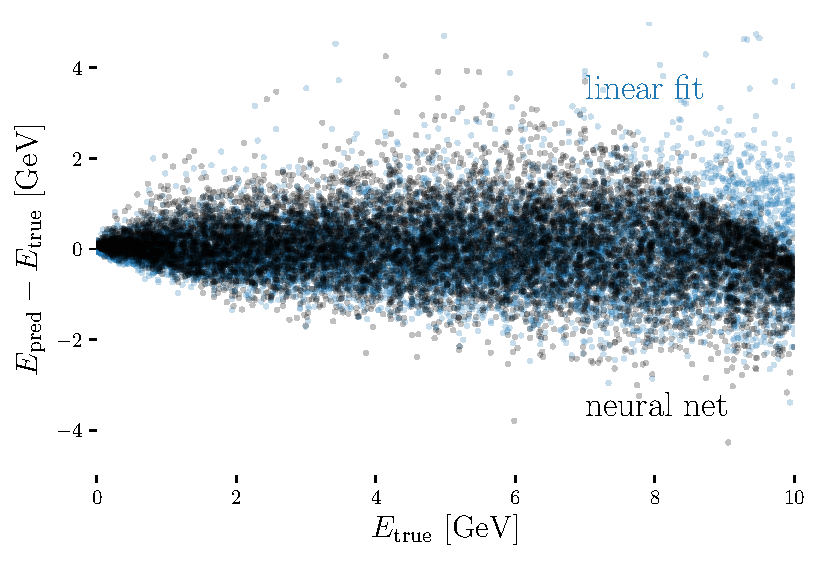
\includegraphics[width=1.1\textwidth]{../first.pdf}
    \end{figure}
  \end{columns}
\end{frame}

\begin{frame}{Data Augmentation}
  \begin{itemize}
  \item flip the data arrays in the y axes
  \item rotate around the x axes
  \item shift in y and z
  \end{itemize}
    \begin{figure}[htp]
      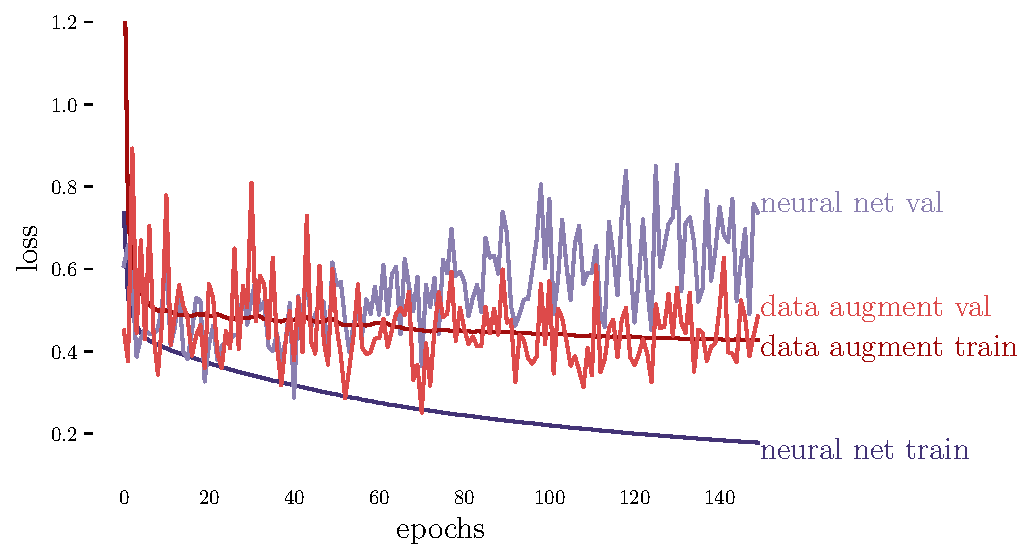
\includegraphics[width=0.8\textwidth]{../data_augment_loss.pdf}
    \end{figure}
\end{frame}


\begin{frame}{Data Augmentation}
  \begin{columns}
    \column{0.5\textwidth}
    \begin{figure}[htp]
      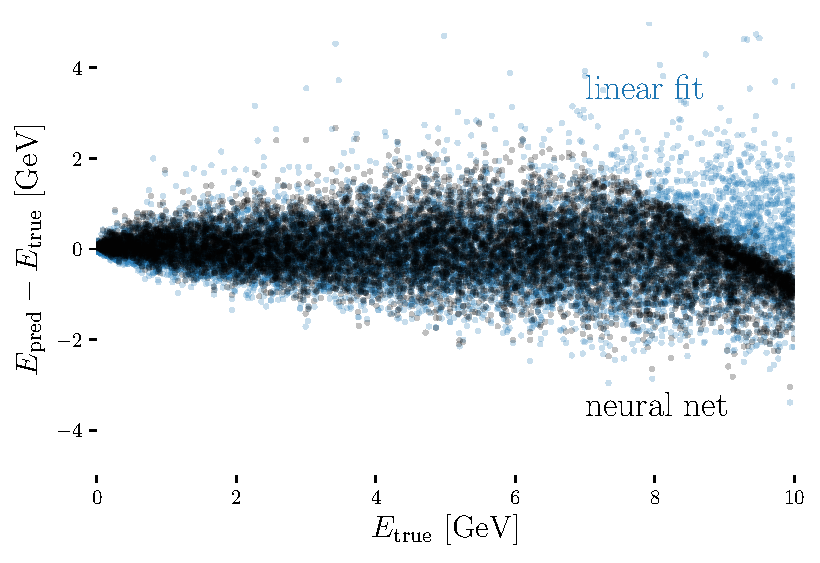
\includegraphics[width=1.1\textwidth]{../data_augment.pdf}
    \end{figure}
    \column{0.5\textwidth}
    \begin{figure}[htp]
      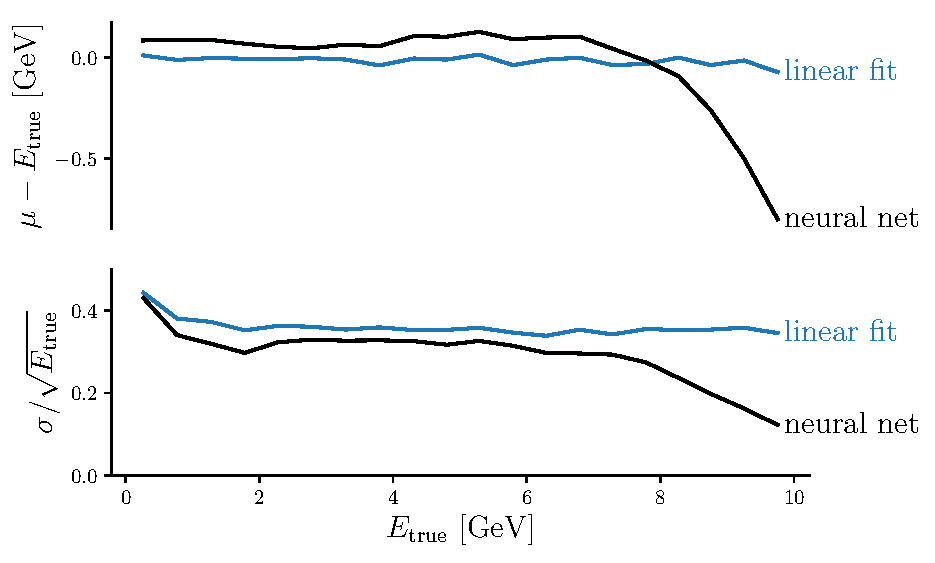
\includegraphics[width=1.1\textwidth]{../data_augment_res.pdf}
    \end{figure}
  \end{columns}
\end{frame}

\begin{frame}{Maximum Likelihood Loss}
Assumption: true values are gaussian distributed with const std $\sigma$
  \begin{align*}
    \text{max likelihood} &= \text{max} \prod \frac{1}{\sqrt{2\pi \sigma^2}} e^{-\frac{(y_{\text{true}}-y_{\text{pred}})^2}{2 \sigma^2}}                          \\
    \Rightarrow \text{max log likelihood} & =\text{max} \sum -\frac{(y_{\text{true}}-y_{\text{pred}})^2}{2 \sigma^2} - \ln(\sqrt{2\pi \sigma^2})                  \\
                                          & =-\text{max} \sum\frac{(y_{\text{true}}-y_{\text{pred}})^2}{\cancel{2 \sigma^2}} - \cancel{\ln(\sqrt{2\pi \sigma^2})} \\
                                          & = \text{min} \sum (y_{\text{true}}-y_{\text{pred}})^2
  \end{align*}
\end{frame}

\begin{frame}{Maximum Likelihood Loss}
  \begin{textblock*}{150pt}(30pt,35pt)
      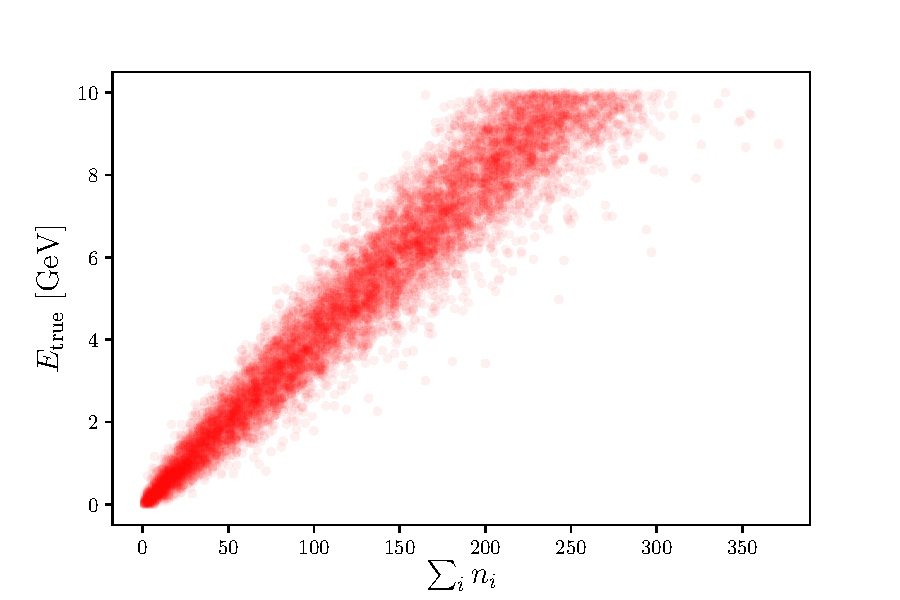
\includegraphics[width=\textwidth]{../e-vs-sum_n.pdf}
  \end{textblock*}
  \begin{textblock*}{150pt}(175pt,35pt)
    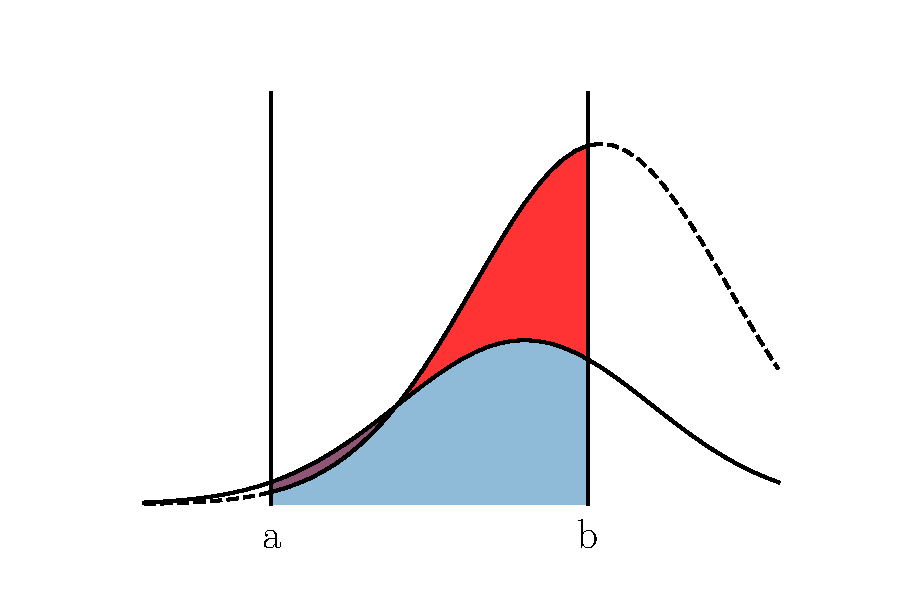
\includegraphics[width=\textwidth]{./gaussian_shift.pdf}
  \end{textblock*}

  \begin{textblock*}{150pt}(5pt,140pt)
    \begin{align*}
      \Rightarrow \text{max log likelihood} = \text{min} \sum& \ln(\frac{\text{Norm}(y_{\text{true}} | y_{\text{pred}}, \sigma)}{\int^b_a \text{Norm}(y_{\text{true}} | y_{\text{pred}}, \sigma)})\\
                                            =\text{min} \sum& \frac{(y_{\text{true}}-y_{\text{pred}})^2}{2 \sigma^2}\\
   &+\ln(\frac{1}{2} \left(\text{erf}(\frac{y_{\text{pred}}-a}{\sqrt{2}\sigma}) - \text{erf}(\frac{y_{\text{pred}}-b}{\sqrt{2}\sigma})\right))
    \end{align*}
  \end{textblock*}
\end{frame}

\begin{frame}{Maximum Likelihood Loss}
  \begin{textblock*}{150pt}(150pt,55pt)
    $\sigma = 0.31 \sqrt{y_{\text{true}}}$
  \end{textblock*}
  \begin{columns}
    \column{0.5\textwidth}
    \begin{figure}[htp]
      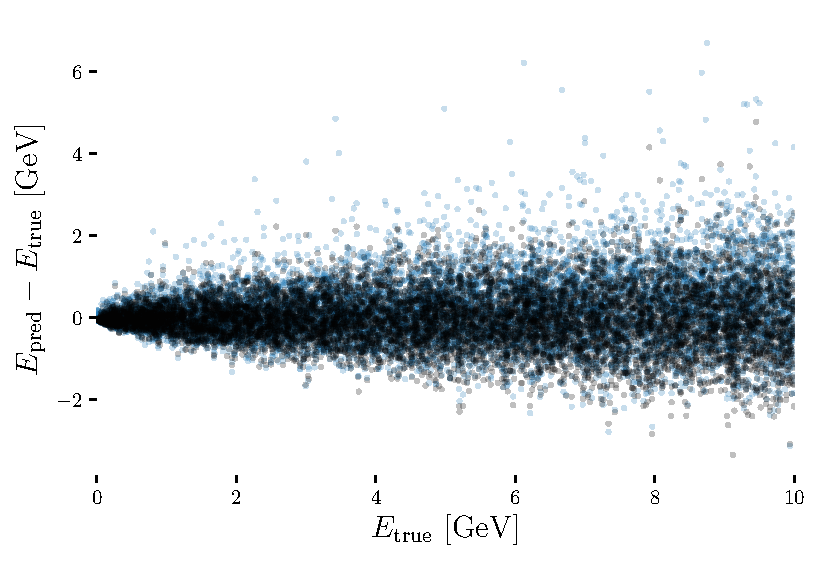
\includegraphics[width=1.1\textwidth]{../likelihood.pdf}
    \end{figure}
    \column{0.5\textwidth}
    \begin{figure}[htp]
      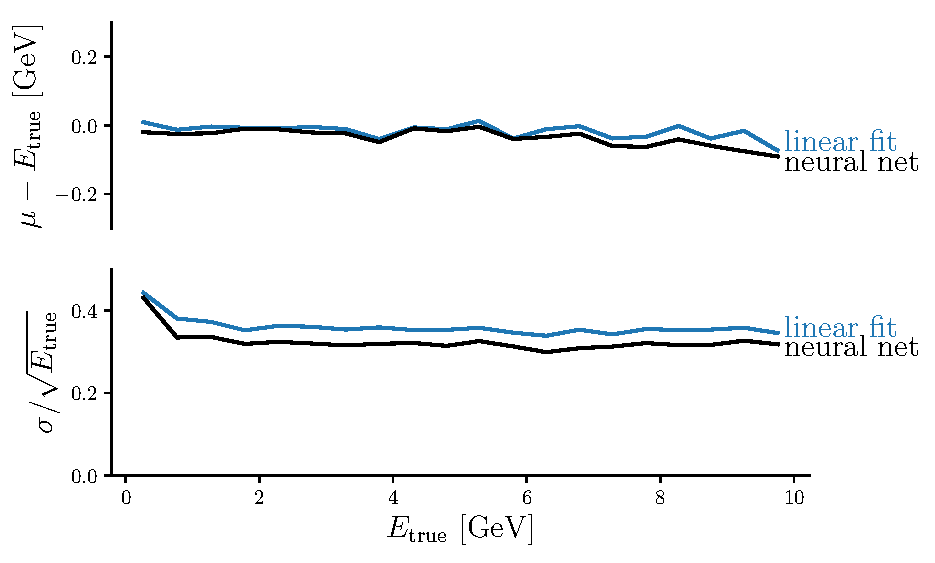
\includegraphics[width=1.1\textwidth]{../likelihood_res.pdf}
    \end{figure}
  \end{columns}
\end{frame}

\begin{frame}{Adversarial Training}
  \usetikzlibrary{arrows}
  \def\layersep{1cm}
  \begin{textblock*}{150pt}(0pt,55pt)
    \small
    \begin{tikzpicture}[shorten >= 1pt, ->, node distance=\layersep,scale=.60]
      \tikzstyle{neuron} = [circle, minimum size=0.25cm, draw=black!20, line width=0.3mm, fill=white]

      % Classifier f
      \node at (2,0) {Classifier $f$};
      \draw (-1,-0.5) rectangle (4,-5.5);

      \path[->, shorten >= 0pt] (-2,-3) edge (-1,-3);
      \node[left] at (-2,-3) {$X$};

      \path[-o, shorten >= 0pt] (1.5,-6.5) edge (1.5,-5.5);
      \node[below] at (1.5,-6.5) {$\theta_f$};

      \path[->, shorten >= 0pt] (3.5,-3) edge (6.5,-3);
      \node[above] at (5.25,-3) {$f(X;\theta_f)$};

      \path[dashed,-] (5.25,-3) edge (5.25,-6.5);
      \node[below] at (5.25,-6.5) {${\cal L}_f(\theta_f)$};

      \foreach \name / \y in {1,...,3}
      \node[neuron] (f-I-\name) at (-0.5,-1-\y) {};

      \foreach \name / \y in {1,...,5}
      \node[neuron] (f-H1-\name) at (-0.5cm+\layersep,-\y cm) {};
      \foreach \name / \y in {1,...,5}
      \node[neuron] (f-H2-\name) at (-0.5cm+3*\layersep,-\y cm) {};

      \node[neuron] (f-O) at (-0.5cm+4*\layersep,-3cm) {};

      \foreach \source in {1,...,3}
      \foreach \dest in {1,...,5}
      \path[black] (f-I-\source) edge (f-H1-\dest);

      \foreach \source in {1,...,5}
      \path[black] (f-H2-\source) edge (f-O);

      \node[black] at (1.5,-3) {...};

      % Adversary r
      \node at (11.75,0) {Adversary $r$};
      \draw (6.5,-0.5) rectangle (11.5,-5.5);

      \node[above] at (13.25,-2) {$\gamma_1(f(X;\theta_f);\theta_r)$};
      \path[-o, shorten >= 0pt] (11,-2.0) edge (15,-2.0);
      \node[above] at (13.25,-3) {$\gamma_2(f(X;\theta_f);\theta_r)$};
      \path[-o, shorten >= 0pt] (11,-3) edge (15,-3);
      \node[above] at (13.25,-4) {$\dots$};
      \path[-o, shorten >= 0pt] (11,-4) edge (15,-4);

      \path[-o, shorten >= 0pt] (9,-6.5) edge (9,-5.5);
      \node[below] at (9,-6.5) {$\theta_r$};

      \foreach \name / \y in {1,...,1}
      \node[neuron] (r-I-\name) at (7,-2-\y) {};

      \foreach \name / \y in {1,...,5}
      \node[neuron] (r-H1-\name) at (7cm+\layersep,-\y cm) {};
      \foreach \name / \y in {1,...,5}
      \node[neuron] (r-H2-\name) at (7cm+3*\layersep,-\y cm) {};

      \node[neuron] (r-O1) at (7cm+4*\layersep,-2cm) {};
      \node[neuron] (r-O2) at (7cm+4*\layersep,-3cm) {};
      \node[neuron] (r-O3) at (7cm+4*\layersep,-4cm) {};

      \foreach \source in {1,...,1}
      \foreach \dest in {1,...,5}
      \path[black] (r-I-\source) edge (r-H1-\dest);

      \foreach \source in {1,...,5}
      \path[black] (r-H2-\source) edge (r-O1);
      \foreach \source in {1,...,5}
      \path[black] (r-H2-\source) edge (r-O2);
      \foreach \source in {1,...,5}
      \path[black] (r-H2-\source) edge (r-O3);

      \node[black] at (9,-3) {...};

      \draw (15,-1.5) rectangle (18,-4.5);
      \path[->, shorten >= 0pt] (16.5,-0.5) edge (16.5,-1.5);
      \node[above] at (16.5,-0.5) {$Z$};
      \path[->, shorten >= 0pt] (16.5,-4.5) edge (16.5,-5.5);
      \node[below] at (16.5,-5.5) {$p_{\theta_r}(Z|f(X;\theta_f))$};
      \node at (16.5,-3) {${\cal P}(\gamma_1, \gamma_2, \dots)$};

      \draw[dashed,-] (16.5,-5) -| (12.75,-6.5);
      \node[below] at (12.75,-6.5) {${\cal L}_r(\theta_f, \theta_r)$};

    \end{tikzpicture}
  \end{textblock*}
  \begin{textblock*}{400pt}(100pt,220pt)
    $ E_\lambda(\theta_f, \theta_r) = {\cal L}_f(\theta_f) - \lambda {\cal L}_r(\theta_f, \theta_r)$
  \end{textblock*}

  \begin{textblock*}{400pt}(10pt,250pt)
    \small G. Louppe, "Learning to Pivot with Adversarial Networks", 1611.01046
  \end{textblock*}
\end{frame}

\begin{frame}{Adversarial Training}
  \begin{itemize}
  \item R estimates $y_{\text{true}}$ given $\frac{y_{\text{true}}-D(X)}{\sqrt{y_{\text{true}}}}$
  \end{itemize}
  \begin{columns}
    \column{0.5\textwidth}
    \begin{figure}[htp]
      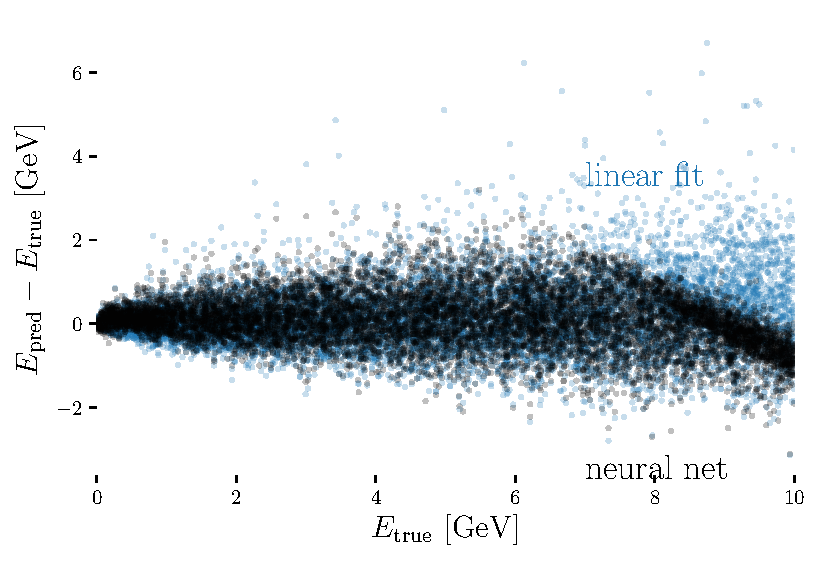
\includegraphics[width=1.1\textwidth]{../adversarial.pdf}
    \end{figure}
    \column{0.5\textwidth}
    \begin{figure}[htp]
      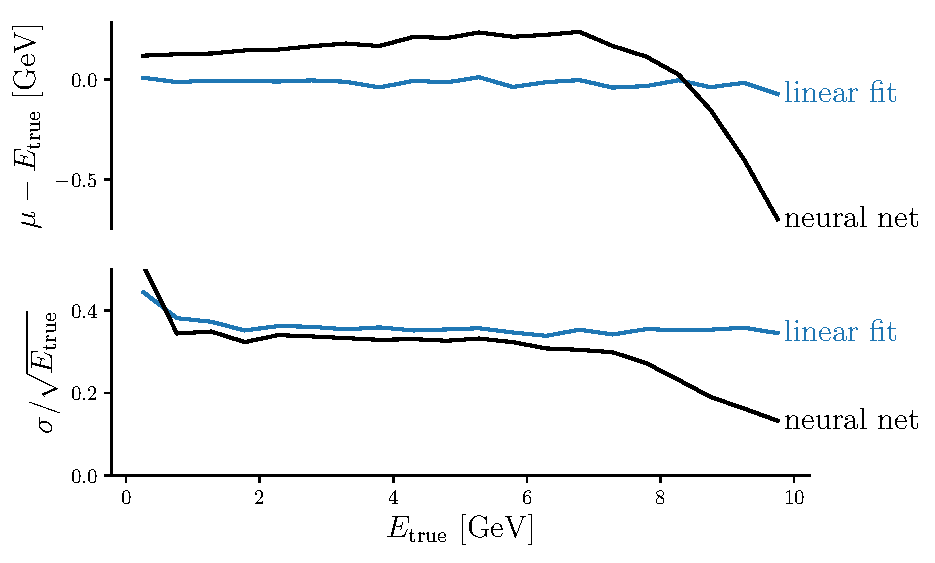
\includegraphics[width=1.1\textwidth]{../adversarial_res.pdf}
    \end{figure}
  \end{columns}
\end{frame}

\begin{frame}{Summary}
  \begin{itemize}
  \item The usage of neural nets at analyzing calorimeter data
  \item Data augmentation is good tool for preventing overfitting in calorimeter data
  \item Two different ways of targeting systematic errors in neural nets
  \item The presented neuralnet performs $\approx 10\%$ better than a linear fit
  \item In this setup the usage of a maximum likelihood loss performs better than
    the adversarial approach
  \end{itemize}
\end{frame}

\end{document}
